\documentclass[portrait,a0,final]{a0poster}
\usepackage{booktabs, tikz, multicol, float, subcaption}
\usetikzlibrary{arrows}
\usepackage[english]{babel}
\floatplacement{figure}{H}
\floatplacement{table}{H}
\usepackage[margin={6cm,6cm}]{geometry}
\usepackage[parfill]{parskip}  %avoid indenting first line of paragraph
\usepackage{enumitem} 
\setlist[enumerate]{itemsep=0mm}
\usepackage{lettrine}
\usepackage{type1cm} % scalable fonts
 
\begin{document}
\bibliographystyle{CIM14}

%FONTS USED
\newcommand{\TITLE}{\VeryHuge \color{red}\sffamily}
\newcommand{\SECTION}{\LARGE \color{red}\sffamily}
\newcommand{\BIG}{\Large \color{black}\sffamily}
\newcommand{\BIGRED}{\Large \color{red}\sffamily}
\newcommand{\NORMAL}{\large \color{black}\sffamily}
\newcommand{\SMALL}{\small \color{black}\sffamily}
\newcommand{\SMALLRED}{\small \color{red}\sffamily}

%\newcommand{\newCommandName}{text to insert}
%Then you can just use \newCommandName{} in the text
%eg. \NORMAL{}

%tikstyles (used by several figures)
%%%%%%%%%%%%%%%%%%%%
\tikzstyle{figureBox} = [fill=white!20, draw=black, thick,
    rectangle, rounded corners=10pt,inner sep=1cm, inner ysep=1cm]
\tikzstyle{textBox} = [fill=orange!20, draw=black, thick,
    rectangle, rounded corners=10pt, inner sep=1cm, inner ysep=1cm]

\begin{center}
\TITLE{}
\textbf{Haptic pattern representation using\\music technologies}\\
\vspace{2em}
\end{center}

\setlength{\columnsep}{2cm}
\begin{multicols}{2}

\begin{center}
\BIG{}
\textbf{Michael Cumming, Adam Tindale, Sara Diamond\\
OCAD University, Toronto, Canada}\\
mcumming@ocadu.ca,
atindale@faculty.ocadu.ca,
sdiamond@ocadu.ca\\
\end{center}
\vspace{1em}

\begin{figure}[H] \centering
\includegraphics[width=0.12\textwidth]{graphicsPoster/OCAD_Logo.png}
\end{figure}
%\vspace{-2em}

\NORMAL{}
\lettrine[lines=2,slope=-4pt,nindent=-4pt]{W}{e} are developing a wrist-wearable, quasi-musical device with vibrotactile arrays, which integrates with a transmedia gaming app on an accompanying smartphone. The main purpose of the wrist device is to register hand gestures and provide clues and notifications for the game player. The vibrotactile arrays also provide pleasant sensual stimulation. We propose that standard musical notation is an appropriate way to program activation patterns for these arrays in a standardized way.\\

%TEXT BOX What is the Problem?
\begin{center}
\begin{tikzpicture}
\node [textBox] (box){ % or figureBox
\begin{minipage}{0.45\textwidth}
\SECTION{}
\textbf{What is the problem?}
\BIG{}
\begin{itemize}
\item How to author interesting and functional vibrating patterns for devices with low resolution \textit{vibrotactile} arrays
\item How to align these patterns with the configuration of the device
\end{itemize}
\end{minipage}};
\end{tikzpicture}
\end{center}
\vspace{2em}


\begin{figure}%[H]
\centering
\includegraphics[width=0.15\textwidth]{graphics/bracelet-02.png}
%caption{Bracelet design with 2x5 tactor array.}
\end{figure}
%\vspace{-1em}
\begin{center}
\NORMAL{}
\textbf{Vibrotactile band with a 2x5 vibe motor array.}
\end{center}


%TEXT BOX Why do this?
\begin{center}
\begin{tikzpicture}
\node [textBox] (box){ % or figureBox
\begin{minipage}{0.45\textwidth}
\SECTION{}
\textbf{Why do this?}
\BIG{}
\begin{itemize}
\item Notification and stimulation from such bands could enrich transmedia narratives and gaming experiences 
\item Touch, vibration and rhythm are important sensual modalities
\item Authoring rhythmic patterns using music notation is efficient and has a long history


\end{itemize}
\end{minipage}};
\end{tikzpicture}
\end{center}
%\vspace{-2em}

%TEXT BOX
\begin{center}
\begin{tikzpicture}
\node [textBox] (box){ % or figureBox
\begin{minipage}{0.45\textwidth}
\SECTION{}
\textbf{Results}
\BIG{}
\begin{itemize}
\item Standard music notation is typically two-dimensional: x-axis handles time, y-axis is pitch (and z-axis is unused)
\item Physical adjacencies of musical instruments are usually not represented in their notation, therefore, authoring for 2D arrays is not straightforward. Multiplication of parts and staves seems the simplest [naive] approach 
\item Standard music notation provides a nuanced, graphical representation for rhythmic events, which is hugely useful for our purposes.
\end{itemize}
\end{minipage}};
\end{tikzpicture}
\end{center}
%\vspace{-2em}

%Music notation is a finely structured notational system. It requires an expert-level of competence to read its finest levels of detail, however, this type of expertise is not hard to find in cultures where notated musical composition and performance is well-established. What is much less common is cross-expertise in both music notation and vibrotactile technologies. Designing interesting and functionally useful patterns for vibrotactile devices is obviously a new field. Standard musical notation includes many dimensions but in its standard forms does not easily lend itself to inclusion of additional non-musical dimensions such as required for the specification of 2 and 3D spatial patterns. These sorts of patterns are important to represent for vibrotactile devices.\\

\NORMAL{}
\textbf{Acknowledgements}\\
\SMALL{}
This work has been supported by the International Science and Technology Partnerships Canada Inc (ISTP) on the project \textit{Multi-platform Game Distribution System for Popular and Experimental Technologies} (MGDS-PET) and by grants from the National Sciences and Engineering Research Council of Canada (NSERC). We would also like to thank Xenophile Media Inc., Vicki Clough, Shin-you Hou, Tegan Power, Ryan Maksymic and Takis Zourntos for the their help in the development of this project.\\
%\vspace{-2em}
\begin{figure}[H] \centering
\includegraphics[width=0.1\textwidth]{graphics/ISTP_logo.png}
\hspace{2em}
\includegraphics[width=0.1\textwidth]{graphics/nserc_logo_color.png}
\end{figure}


%\NORMAL{}
%\textbf{Basic mapping conventions}\\
%\SMALL{}
%\begin{itemize}
%\item Represent time horizontally from left to right. Notes to the right occur later.
%\item A note represents an activation of a component. A component can be of several types (vibe motor, LED, etc.). Place notes on normal, five line staves.
%\item Represent note durations by note type (for example, quarter, half and whole notes), dots and by ties between notes of the same pitch.
%\item If notes are pitched, indicate their pitch through their vertical placement on a staff. If notes are unpitched, represent different components (e.g. different types of vibe motors or LEDs) using various note heads or annotations.
%\item Different \textit{parts} are on separate staves. One tactor type playing the same notes at the same time represents playing in \textit{unison}. For example, eight vibe motors playing in unison can be represented as one part.
%\item Simultaneous notes, or \textit{chords}, are stacked vertically as in music notation.
%\end{itemize}

%\SECTION{}
%\textbf{Why?}\\
%\NORMAL{}

%%coloured box with text
%%\tikzstyle{mybox} = [draw=black, fill=orange!20, thick,
%   % rectangle, rounded corners, inner sep=1cm, inner ysep=1cm]
%\begin{center}
%\begin{tikzpicture}
%\node [textBox] (box) {
%\begin{minipage}{0.45\textwidth}
%
%\normalsize \color{black}
%\textbf{Use cases for wrist-wearable device}
%\begin{enumerate}
%  \item Interpret wrist gestures and recognize overall physical activity of the wearer (using the microcontroller's accelerometer),
%  \item notify the wearer when crystals and treasures are earned,
%  \item offer vibrotactile clues about where crystals and treasures can be found, and
%  \item provide aesthetically attractive and evocative vibe and light displays corresponding to narrative points in a story.
%\end{enumerate}
%
%\end{minipage}};
%\end{tikzpicture}
%\end{center}
    
%TEST BOX TEMPLATE vvvvvvvvvvvvvv
%\begin{center}
%\begin{tikzpicture}
%\node [textBox] (box){ % or figureBox
%\begin{minipage}{0.45\textwidth}
%    
%%Content goes here:
%TEXT BOX TEMPLATE
%    
%\end{minipage}};
%\end{tikzpicture}
%\end{center}
%TEST BOX TEMPLATE ^^^^^^^^^^^^^^

%We also need to translate the nomenclature from the domain of wrist wearables to that of music notation. This mapping is shown in the following table:
%
%\begin{center}
%\begin{tikzpicture}
%\node [textBox] (box){ % or figureBox
%\begin{minipage}{0.45\textwidth}
%    
%\begin{table}[H]
%\SMALL{}\sffamily
%%\caption{Vibrotactile vs Music notation terms}
%\normalsize
%%\centering
%\begin{tabular}{@{}ll@{}}
%%\toprule
%\textbf{Vibrotactile term} & \textbf{Music notation term}\\ 
%\midrule
%Activation of one component & Note \\
%Activation duration & Note duration \\
%Frequency of an activation & Pitch \\
%One type of component & Instrument \\
%Series of activations for one component & Part \\
%Simultaneous activations w/ multiple pitches & Chord \\
%Integrated series of activations & Composition \\
%%\bottomrule
%\end{tabular}
%\end{table}
%    
%\end{minipage}};
%\end{tikzpicture}
%\end{center}

%Therefore, the basic components of music are present even with a wrist-wearable vibrotactile device that does not, at first, seem to have a musical aspect: \textit{notes} with durations, pitched notes played on various discrete \textit{instruments} (vibe motors and LED lights), various \textit{parts,} or \textit{voices,} played in polyphonic \textit{compositions} and the dynamics of various parts playing together. \\

%\normalsize \color{red}
%\textbf{Pitch}
%\SMALL{}
%Vertical placement for normal, pitched notes in music notation indicates their pitch. Pitch differentials are possible with tactors, as their frequency can be modelled using standard pulse-width modulation (PWM) techniques \cite{lindeman2006wearable}. The pitch of a note is one of its primary psychoacoustic attributes, along with its duration, loudness and timbre. Unpitched notes are those for which the frequency is indeterminate, too complex or unrelated to the pitch contours of melodic or harmonic parts. The perception of pitch in vibrotactile devices differs from that of normal acoustic instruments. The number of frequency differences is much reduced and depends on amplitude. The skin's maximal frequency response occurs around 250 Hz \cite{gunther2003cutaneous}. There may be as few as five frequency distinctions possible with cutaneous perception, or as many as ten \cite{van2003distilling}.  So, the chromatic range of pitches and frequencies over many octaves as normally represented using music notation is not suitable for cutaneous perception, it appears that some, relatively minor variation in pitch is possible. These considerations would seem not to preclude the use of music notation for our purposes -- the use of notes to represent non-aural sensory expression.\\

%\normalsize \color{red}
%\textbf{Intensity}
%\SMALL{}
%The intensity of a vibrotactile stimulus is defined by the strength or magnitude of its vibration. As with aural music, suitable intensities for vibrotactile devices range from those that are barely perceptual to those that become uncomfortable. Classic work in this area was done by measuring Weber fractions and just noticeable differences (JNDs). Frequency and intensity parameters interact in vibrotactile studies in that differences can be ascribed to combinations of parameters \cite{van2003distilling}. The intensity threshold is adaptable and depends on a variety of parameters such as actuator used, location of the stimulation, person, or frequency of the vibration \cite{jonas2008tactile}. Geldard discovered that while we can discriminate 15 levels of vibrotactile stimuli intensity but that no more than three intensity levels can be identified absolutely \cite{geldard1960some}. Considerations of the amplitude envelope (amplitude, delay, sustain, release, or ADSR) and with amplitude modulations such as tremolo or pitch modulations like vibrato  are also important with vibrotactile stimulation \cite{gunther2003cutaneous}.\\

%\normalsize \color{red}
%\textbf{Duration}
%\SMALL{}
%The term duration refers to the length of the tactile stimulus -- from onset to the termination of the stimulus. There exist various reference values for duration and is generally measured in milliseconds \cite{jonas2008tactile}. It is important to ensure that the individual vibrotactile stimuli are within a reasonable range of durations. Geldard found that stimuli duration roughly between 0.1 and two seconds is reasonable \cite{geldard1960some}. If vibrotactile notes are of short duration they are perceived as sharp taps or jabs in the skin \cite{gunther2003cutaneous}, while stimuli that lasted longer than the upper limit of two seconds delays communication \cite{jonas2008tactile}. Dynamic properties of a vibration signal such as its envelope, duration, and the presence of masking stimuli may also affect perceptual threshold levels \cite{birnbaum2007musical}.\\

%\normalsize \color{red}
%\textbf{Spatial patterns and vibrotactile clues}
%\SMALL{}
%As noted above one of the primary use cases for our vibrotactile device is offer vibrotactile clues about where crystals and treasures can be found within transmedia-inspired gameplay. These clues are intended to provide the following messages to the game-player: \textit{Go this way / don't go that way}, and 
%\textit{You're getting warmer / you're getting colder}. These are spatial and metaphorical in nature and allude to navigating through some kind of virtual space. Pan�els discusses vibrotactile design for metaphorical patterns such as \textit{turn back} on devices that have actuators with spatial patterns, but does it in a non-musical context \cite{paneels2013tactiped}. Ideally these gameplay clues are either self-explanatory or easy for the player to learn. A vibrotactile device having a series of tactors activating in the intended direction might be a good first step in suggesting \textit{go this way}, much like a flashing series of traffic lights scrolling to the right suggest proceed to the right (Figure ~\ref{fig:tactorArray}). To test such intuitions requires additional study. One should also note that wrist-worn devices can be oriented in various ways, depending on wrist position.\\

%Music as it is commonly notated does not lend itself to these sorts of concepts or metaphors. Although music that has spatial aspects is common, such as the surround sound of Thomas Tallis' \textit{Spem in Alium} [1570], or the call and response of antiphonal works, standard music notation tends not to focus on the specification of spatial aspects in music performance -- even though aural perception is intensely spatial. In ensembles, sections of instruments playing the same parts are usually placed together but this is a performance convention and is usually outside of the notation itself. Therefore, it is unclear at first what notated music that could be interpreted as \textit{go this way}, or \textit{you're getting warmer} might look like.\\


%\begin{figure}[H]
%\definecolor{light-gray}{gray}{0.85}
%\definecolor{med-gray}{gray}{0.65}
%\definecolor{dark-gray}{gray}{0.35}
%  	
%	%\begin{tikzpicture}[scale=2.0]
%	\begin{center}
%	\begin{tikzpicture}[scale=2]
%	%arrow on top:
%	\draw[thick,->, line width=2pt] (0.5,2.5) -- (4.5,2.5);
%	%curved arrows:
%	%\draw[thick,->,>=angle 90, line width=2pt, shorten >=10pt, shorten <=10pt] 
%		%(4.5,1.5) .. controls (9,3) and (-4,3) .. (0.5,1.5);
%	%\draw[thick,->,>=angle 90, line width=2pt, shorten >=10pt, shorten <=10pt] 
%		%(4.5,0.5) .. controls (9,-1) and (-4,-1) .. (0.5,0.5);
%	%grid:
%	\draw[step=1cm,gray,very thin] (0,0) grid (5,2);
%	%bottom row:
%	\filldraw[fill=dark-gray, draw=black] (0.5,0.5) circle (0.12cm);
%	\filldraw[fill=white, draw=black] (1.5,0.5) circle (0.12cm);
%	\filldraw[fill=white, draw=black] (2.5,0.5) circle (0.12cm);
%	\filldraw[fill=white, draw=black] (3.5,0.5) circle (0.12cm);
%	\filldraw[fill=white, draw=black] (4.5,0.5) circle (0.12cm);
%	%top row:
%	\filldraw[fill=dark-gray, draw=black] (0.5,1.5) circle (0.12cm);
%	\filldraw[fill=white, draw=black] (1.5,1.5) circle (0.12cm);
%	\filldraw[fill=white, draw=black] (2.5,1.5) circle (0.12cm);
%	\filldraw[fill=white, draw=black] (3.5,1.5) circle (0.12cm);
%	\filldraw[fill=white, draw=black] (4.5,1.5) circle (0.12cm);
%
%	\end{tikzpicture}
%  	%\caption{2x5 array of tactors with directional activation.}
%  	\label{fig:tactorArray}
%
%\end{figure}
%\textbf{2x5 array of tactors with directional activation.}
%\end{center}

%\bigskip
%\bigskip

%vvvvvvvvv%%%%%%%%%%%%%%%%%%%%%%%%%%%%%%%%%%
%http://tex.stackexchange.com/questions/18363/diagrams-package-that-allows-to-draw-computer-buffers-memory-diagrams

%\begin{center}
%\begin{tikzpicture}[>=latex,font=\sffamily,semithick,scale=3]
%    \fill [green!25] (0,0) -- (67.5:1) arc [end angle=-22.5, start angle=67.5, radius=1] -- cycle;
%    \draw [thick] (0,0) circle (1);
%    \foreach \angle in {90,67.5,...,-67.5}
%        \draw (\angle:1) -- (\angle-180:1);
%    \node [circle,thick,fill=white,draw=black,align=center,minimum size=3cm] at (0,0) {FIFO as a\\Circular Buffer};
%    \draw [<-] (56.25:1) -- (56.25:1.25) -- +(.333,0)
%        node [right,inner xsep=.333cm] (Head) {Head (extract)};
%    \draw [<-] (-33.75:1) -- (-33.75:1.25) -- +(.333,0)
%        node [right,inner xsep=.333cm] (Tail) {Tail (insert)};
%    \draw [->,shorten >=5pt,shorten <=5pt] (Tail.west) to [bend right] 
%        node [midway,sloped,above,allow upside down] {\footnotesize 4\,bytes in FIFO}
%    (Head.west);
%\end{tikzpicture}
%\par
%\textbf{Circular array 1}
%\end{center}

%\begin{center}
%\begin{tikzpicture}
%\draw [thick] (0,0) circle (4);
%\draw [thick] (0,0) circle (5);
%\foreach \angle in {0,60,...,300}
%	\draw [thick, fill=black, rotate=\angle, shift={(5, 0)}] (0,0) circle (0.25);
%\foreach \angle in {0,60,...,300}
%	\draw [thick, fill=black, rotate=\angle, shift={(4, 0)}] (0,0) circle (0.25);
%\end{tikzpicture}
%\par
%\textbf{Circular array of tactors.}
%\end{center}

%\bigskip
%\bigskip


%\par
%\bigskip35

%\begin{center}
%\begin{tikzpicture}[>=latex,font=\sffamily,every node/.style={minimum width=2cm, minimum height=2cm, outer sep=0pt, draw=black, thick}]
%        \node at (0,0) (A) {1};
%        \node [anchor=west] at (A.east) (B) {2};
%        %\draw [anchor=west] at (A.east) circle (0.25);
%        \node [anchor=west] at (B.east) (C) {3};
%        \node [anchor=west] at (C.east) (D) {4};
%        \node [anchor=west] at (D.east) (E) {5};
%        \node [anchor=west] at (E.east) (F) {6};
%        \draw [thick,->,>=angle 90, line width=2pt, shorten >=5pt, shorten <=5pt] 			(F.south) -- +(0,-1em) -| (A);
%\end{tikzpicture}
%\par
%\textbf{Linear array of tactors.}
%\end{center}
%\bigskip
%\bigskip
%^^^^^^^^^%%%%%%%%%%%%%%%%%%%%%%%%%%%%%%%%%


%%%%%%%%%%%%%%%%%%%%%%%%%%%%%%%%%%%%%%%
%\BIGRED{}
%\textbf{Controlling Components using Musical Notation}
%\SMALL{}
%%%%%%%%%%%%%%%%%%%%%%%%%%%%%%%%%%%%%%%

%\normalsize \color{red}
%%\textbf{Music with one spatial dimension (1D = linear)}\\
%\SMALL{}
%Following this line of reasoning, music with one spatial dimension is that which instruments follow some kind of spatial linear progression along one line, such as pan or a sweep. Figure ~\ref{fig:arrowsMoving00}. shows one vibe motor activating in a simple rhythm with a simple, rhythmic pitch change. 
%By the conventions of music notation it is clear that a regular rhythm is being represented. Of course, to appreciate this requires at least a rudimentary knowledge of music notation. To design a pattern of similar rhythmic complexity by means other than music notation would likely be more difficult. \\

%ZERO DIM
\begin{center}
\begin{tikzpicture}
\node [figureBox] (box){ % or textBox
\begin{minipage}{0.45\textwidth}
\begin{center}
\BIGRED{} 
\textbf{Device with no spatial dimension (0D = point)}\\

\vspace{1em}
\SMALL{}
\begin{tikzpicture}[scale=2]
%grid
\draw[step=1cm,gray,very thin] (0,0) grid (1,1);
%circles:
\filldraw[fill=blue, draw=black] (0.5,0.5) circle (0.12cm);
%\draw[very thin] (0.5,0.5) circle (0.2cm);
%\draw[very thin] (0.5,0.5) circle (0.35cm);
\end{tikzpicture}\\
\textbf{Device with a single vibe motor}

\vspace{1cm}
%bottom figure (musical staff)
\begin{figure}[H] \centering
        \includegraphics[width=0.65\textwidth]{graphicsPoster/arrowsMoving-00.pdf}
\end{figure}
\textbf{Score for single vibe motor playing a simple `solo' rhythm}\\
\end{center}

\begin{itemize}
\item Time = horizontal axis; rhythmic information as per standard musical notation
\item For most vibe motors pitch remains constant, but intensity can vary; Intensity specified by dynamics markings
\item Vertical position does not vary (y-axis unused, therefore unpitched notation would also be suitable)
\item Information is not very dense (single line score would suffice)
\item \textbf{NEXT STEP} notate for multiple vibe motors
\end{itemize}
\rule{\textwidth}{0.5pt}\\

%ONE DIM, unpitched
\begin{center}
\BIGRED{} 
\textbf{Device with one spatial dimension (1D = linear)}\\
\textbf{Vertical note position maps to five components}\\
\vspace{1em}

\SMALL{}
%top diagram
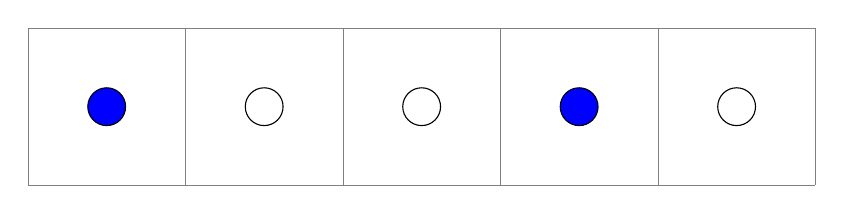
\begin{tikzpicture}[scale=2]
%grid
\draw[step=1cm,gray,very thin] (0,0) grid (5,1);
%bottom row:
\filldraw[fill=blue, draw=black] (0.5,0.5) circle (0.12cm);
\filldraw[fill=white, draw=black] (1.5,0.5) circle (0.12cm);
\filldraw[fill=white, draw=black] (2.5,0.5) circle (0.12cm);
\filldraw[fill=blue, draw=black] (3.5,0.5) circle (0.12cm);
\filldraw[fill=white, draw=black] (4.5,0.5) circle (0.12cm);
\end{tikzpicture}\\
\textbf{Device with a line of vibe motors}.
\vspace{2cm}
%bottom figure (musical staff)
\begin{figure}[H] \centering
        \includegraphics[width=0.8\textwidth]{graphicsPoster/arrowsMoving-00-drumStaff.pdf}
\end{figure}
\textbf{Score for a linear array of five vibe motors}
\end{center}

\begin{itemize}
\item Specifies activations for five, independent vibe motors
\item Each part occupies one staff line (rests are hidden); for unpitched components yet uses five staff lines
\item Vertical staff position specifies vibe motor to activate; top line=1, second line=2, etc; MIDI note $\Rightarrow$ vibe motor
\item \textbf{PROBLEM} Five unpitched parts on one staff are hard to read, especially if rhythms are complex
\item \textbf{NEXT STEP} Make notation less dense and more readable
\end{itemize}
\rule{\textwidth}{0.5pt}\\

%ONE DIM, low density
%bottom figure (musical staff)
\begin{center}
\BIGRED{}
\textbf{Part numbering maps to five components}\\
\vspace{1em}

\SMALL{}
\begin{figure}[H] \centering
        \includegraphics[width=0.55\textwidth, height=.35\textwidth]{graphicsPoster/arrowsMoving-01-drumStaves.pdf}
\end{figure}
\textbf{Score for a linear array of five vibe motors}
\end{center}
\begin{itemize}
\item Specifies activations for five, independent components
\item Five part single-line staff, rhythmic notation 
\item MIDI number derived from part number; this maps to vibe motor address
\item \textbf{NEXT STEP} Make notation suitable for two dimensional arrays of vibe motors
\end{itemize}
\rule{\textwidth}{0.5pt}\\

%TWO DIM
\begin{center}
\BIGRED{} 
\textbf{Device with two spatial dimension (2D = planar)}\\
\vspace{1em}

\SMALL{}
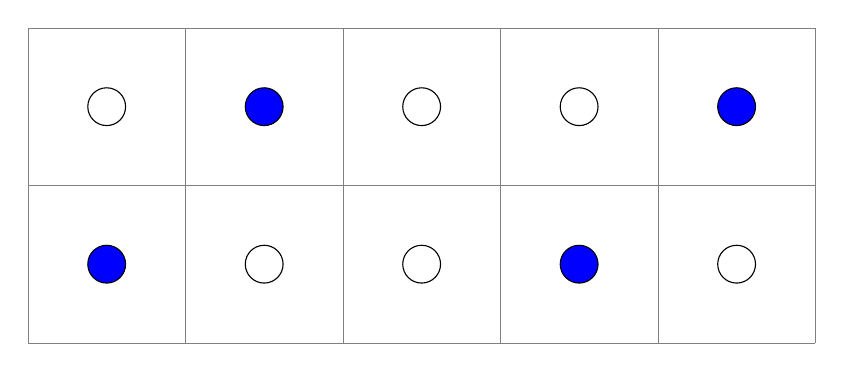
\begin{tikzpicture}[scale=2]
%grid
\draw[step=1cm,gray,very thin] (0,0) grid (5,2);
%top row:
\filldraw[fill=white, draw=black] (0.5,1.5) circle (0.12cm);
\filldraw[fill=blue, draw=black] (1.5,1.5) circle (0.12cm);
\filldraw[fill=white, draw=black] (2.5,1.5) circle (0.12cm);
\filldraw[fill=white, draw=black] (3.5,1.5) circle (0.12cm);
\filldraw[fill=blue, draw=black] (4.5,1.5) circle (0.12cm);
%bottom row:
\filldraw[fill=blue, draw=black] (0.5,0.5) circle (0.12cm);
\filldraw[fill=white, draw=black] (1.5,0.5) circle (0.12cm);
\filldraw[fill=white, draw=black] (2.5,0.5) circle (0.12cm);
\filldraw[fill=blue, draw=black] (3.5,0.5) circle (0.12cm);
\filldraw[fill=white, draw=black] (4.5,0.5) circle (0.12cm);
\end{tikzpicture}\\
\textbf{Device with an array of vibe motors}
\vspace{2cm}

%top score (musical staff)
\begin{figure}[H] \centering
        \includegraphics[width=0.55\textwidth]{graphicsPoster/arrowsMoving-5sysx2lines.pdf}
\end{figure}
\textbf{Score where each staff represents one COLUMN of vibe motors}
\vspace{1em}
%bottom scale (musical staff)
\begin{figure}[H] \centering
        \includegraphics[width=0.6\textwidth]{graphicsPoster/arrowsMoving-2sysx5lines.pdf}
\end{figure}
\textbf{Score where each staff represents one ROW of vibe motors}
\end{center}

\begin{itemize}
\item Time = horizontal, x-axis
\item Ten components need independent addressability 
\item Either five staves (for columns) or two staves (for rows)
\end{itemize}
\end{minipage}};
\end{tikzpicture}
\end{center}

%\begin{figure}[htb]
%    \begin{center}
%        \includegraphics[width=0.4\textwidth]{graphics/scaleArduino-01.pdf}
%    \end{center}
%    \caption{Simple scale for a pitched Arduino component.\label{fig:fig2}}
%\end{figure}

%\begin{figure}[htb]
%    \begin{center}
%        \includegraphics[width=0.4\textwidth]{graphics/drums1-multistaff.pdf}
%    \end{center}
%    \caption{Complex rhythm for three Arduino components.\label{fig:fig4}}
%\end{figure}

%\begin{figure}[htb]
%    \begin{center}
%        \includegraphics[width=0.3\textwidth]{graphics/drums1-simple.pdf}
%    \end{center}
%    \caption{Simple rhythm for two unpitched Arduino components.\label{fig:fig3}}
%\end{figure}

%\begin{figure}[H]
%    \begin{center}
%       \includegraphics[width=0.3\textwidth]{graphics/arrowsMoving-01.pdf}
%  \end{center}
%  \caption{Threes vibes activating sequentially.\label{fig:arrowsMoving01}}
%\end{figure}

%Figure ~\ref{fig:arrowsMoving01}. shows three vibe motors activating in a sequential motion. The motors are arranged along a line and therefore are only one dimensional. Since they are playing the same pitch if the three separate parts where placed on the same staff there would be confusion about which note applies to which motor. Because of their linear placement their pulsation has a directionality. However, this directionality is less apparent in the notation itself. The only indication that Vibe 02 might be located after Vibe 01 is because of the numbering of the score. Yet with vibe bracelets it is desirable to be able to represent two dimensions such that common 2D patterns such as moving sprites, radiating waves and the like can be created across the skin. Is it possible to easily represent the activation of a 2D array of instruments using standard music notation?\\

%\normalsize \color{red}
%\textbf{Music with additional spatial dimensions (2D = planar)}\\
%\SMALL{}
%With pitched notation the pitch, timing and rhythm of the music tends to be its most important aspect. Time occupies the \textit{x} dimension while pitch occupies the \textit{y}. The spatial placement of the instruments playing different parts is less of a concern. You can have many \textit{parts}, or stack notes in \textit{chords} but this seems only to provide you with one additional dimension. With variables outside of standard notation, such as those that can be accessed though midi channels, additional mappable dimensions may be possible but then this becomes similar to using other programming techniques in which dimensions of information are represented using, for instance, multi-dimensional arrays. The clear graphic presentation of standard music notation, which could be so useful in depicting complex music patterns, would then be lost.\\

%\normalsize \color{red}
%Future Work\\
%\SMALL{}
%Our work consists of quick iteration of devices and authoring of activation patterns for several devices. This work is motivated by both research and aesthetic considerations. Pattern authoring depends crucially on the nature of the device being authored for and its purpose. We consider two aspects that seem particularly promising for future development in this area: the design of vibrotactile patterns to enhance and inform transmedia narratives, and the creation of aesthetically appealing vibrotactile patterns in a variety of musical \textit{genres}. We are also interested in ways of packing more information into standard music notation since it provides a means of representing complex patterns of activation in an elegant form.\\

%% REFERENCES
%\bibliography{CIM14_bibliography}
%\bibliographystyle{CIM14}

\end{multicols}
\end{document}
